\documentclass[a4paper,12pt]{article}
\usepackage{geometry}
\usepackage{graphicx}
\geometry{margin=2cm}
\usepackage{array}
\usepackage{booktabs}
\usepackage{fancyhdr}
\usepackage{pdfpages}
\usepackage{float}
\usepackage{hhline}

\title{\Large ELE4116: Electrical Installation Design\\[0.5cm]
\textbf{\Huge Electrical Lighting and Power System Design Concept Note}}
\author{}
\date{}

\begin{document}

\maketitle

\section*{Group Members}
\begin{table}[H]
    \centering
    \begin{tabular}{|l|l|} 
        \hline
        Agaba Derick & 21/U/20627/PS \\
        \hline
        Walyuba Denis & 21/U/0972 \\
        \hline
        Ssenabulya Stuart & 21/U/19348/PSA \\
        \hline
        Mawungu Bashir Kayinda & 21/U/0375 \\
        \hline
        Shawal Mbalire & 21/U/0851 \\
        \hline
        Kivumbi Douglas & 18/U/22545/PS \\
        \hline
        Naluyinda Hajarah & 21/U/07660/PSA \\
        \hline
        Wandera Florence & 21/U/07273/PS \\
        \hline
        Namayanja Pauline & 21/U/19843/PS \\
        \hline
    \end{tabular}
    \label{<label>}
\end{table}

\section{Introduction}
This project involves designing a comprehensive electrical lighting and power system for a residential building, consisting of various functional spaces such as bedrooms, living rooms, kitchens, and bathrooms. Using AutoCAD, the aim is to ensure efficient, safe, and optimized electricity distribution for lighting, power sockets, and the lightning protection system (LPS). The system will adhere to industry standards and regulatory codes.

\section{Project Objectives}
The primary objectives of this project are:
\begin{itemize}
    \item To design an energy-efficient lighting system tailored to meet the functional needs of each room.
    \item To develop an optimized layout for power sockets, ensuring convenient access in all rooms.
    \item To comply with safety standards, allowing for balanced load distribution across circuits.
    \item To provide a clear, detailed schematic that can be readily implemented on-site.
\end{itemize}

\section{Scope of Work}
The scope includes accurately recreating the architectural floor plan in AutoCAD based on the provided layout. The focus will be on:
\begin{itemize}
    \item \textbf{Lighting System}: Placement of energy-efficient LED fixtures suited to room-specific requirements, with a detailed schematic showing connections to switches and the distribution board.
    \item \textbf{Power Sockets}: Positioning of power outlets for convenient access in each room, balanced with circuits to optimize load distribution.
    \item \textbf{Load Estimation}: Total electrical load requirements will be calculated to ensure safety and efficiency in balancing loads across circuits.
\end{itemize}

\section{Methodology}
The project applies to a dual-unit residential building with symmetrical layouts. Each unit contains two bedrooms, a kitchen, a living/dining room, and associated spaces (e.g., bathrooms, storage). The architectural plan measures 21.4m x 12.8m in total.

\subsection{Power Outlet Design for Each Unit}
Based on room function and anticipated usage, the following power outlet allocations are proposed:
\begin{itemize}
    \item Living Room: 4 sockets
    \item Dining Room: 1 socket
    \item Master Bedroom: 2 sockets
    \item Master Bathroom: 1 socket
    \item Children’s Bedroom: 2 sockets
    \item Kitchen: 3 sockets
    \item Dirty Kitchen: 1 socket
\end{itemize}

\subsection{Appliance Load Ratings}
The table below outlines standard appliances and their ratings, used for load calculations in each unit:
\begin{table}[H]
    \centering
    \begin{tabular}{|l|c|c|}
        \toprule
        \textbf{Appliance} & \textbf{Quantity} & \textbf{Power Rating (kW)} \\
        \midrule
        Washing Machine & 1 & 1.5 \\
        Refrigerator & 1 & 0.3 \\
        Water Heater & 2 & 5.0 \\
        Cooker & 1 & 2.0 \\
        Microwave & 1 & 0.8 \\
        Dryer & 1 & 6.0 \\
        Dishwasher & 1 & 1.8 \\
        \bottomrule
    \end{tabular}
    \caption{Standard Appliance Load Ratings}
\end{table}

\section{Lighting Calculation}
The following table details lighting requirements per room, based on dimensions and function:
\begin{table}[H]
    \centering
    \begin{tabular}{|l|c|c|c|c|c|c|}
        \hline
        \textbf{Room} & \textbf{Length(m)} & \textbf{Width (m)} & \textbf{Area(m$^2$)} & \textbf{Lamps} & \textbf{Power(W)} & \textbf{Total(W)} \\
        \hline
        Children’s Bedroom & 4.5 & 3.2 & 14.4 & 1 & 5 & 5 \\
        Living Room & 4.2 & 2.5 & 10.5 & 3 & 10 & 30 \\
        Dining Room & 4.2 & 4.15 & 17.43 & 2 & 5 & 10 \\
        Master Bedroom & 4.5 & 3.3 & 14.85 & 3 & 5 & 15 \\
        Store & 2.0 & 1.5 & 3.0 & 1 & 5 & 5 \\
        Master Bathroom & 3.15 & 1.5 & 4.72 & 1 & 5 & 5 \\
        Kitchen & 3.4 & 2.55 & 8.67 & 1 & 5 & 5 \\
        \hline
    \end{tabular}
    \caption{Lighting Requirements by Room}
\end{table}

\section{Materials and Equipment}
The following materials and equipment are required:
\begin{itemize}
    \item \textbf{AutoCAD Software}: For creating layout and schematic drawings.
    \item \textbf{LED Lighting Fixtures}: Energy-efficient, with a typical rating of 9-12 watts per fixture.
    \item \textbf{Wiring}: Standard residential wiring (e.g., 2.5mm² for sockets, 1.5mm² for lighting circuits).
    \item \textbf{Sockets and Switches}: High-quality, durable outlets for safety.
    \item \textbf{Distribution Board and Circuit Breakers}: Suitable to handle load requirements (6A for lighting circuits, 16A for socket outlets).
    \item \textbf{Protection Equipment}: Including RCDs and surge protectors for safety.
\end{itemize}

\section{Conclusion}
This project aims to deliver a comprehensive and optimized electrical lighting and power system design for a residential building. The use of AutoCAD ensures precise design, and the adoption of energy-efficient LED lighting and strategically placed power sockets enhances functionality. Safety, load balancing, and compliance with electrical codes are emphasized throughout the project.

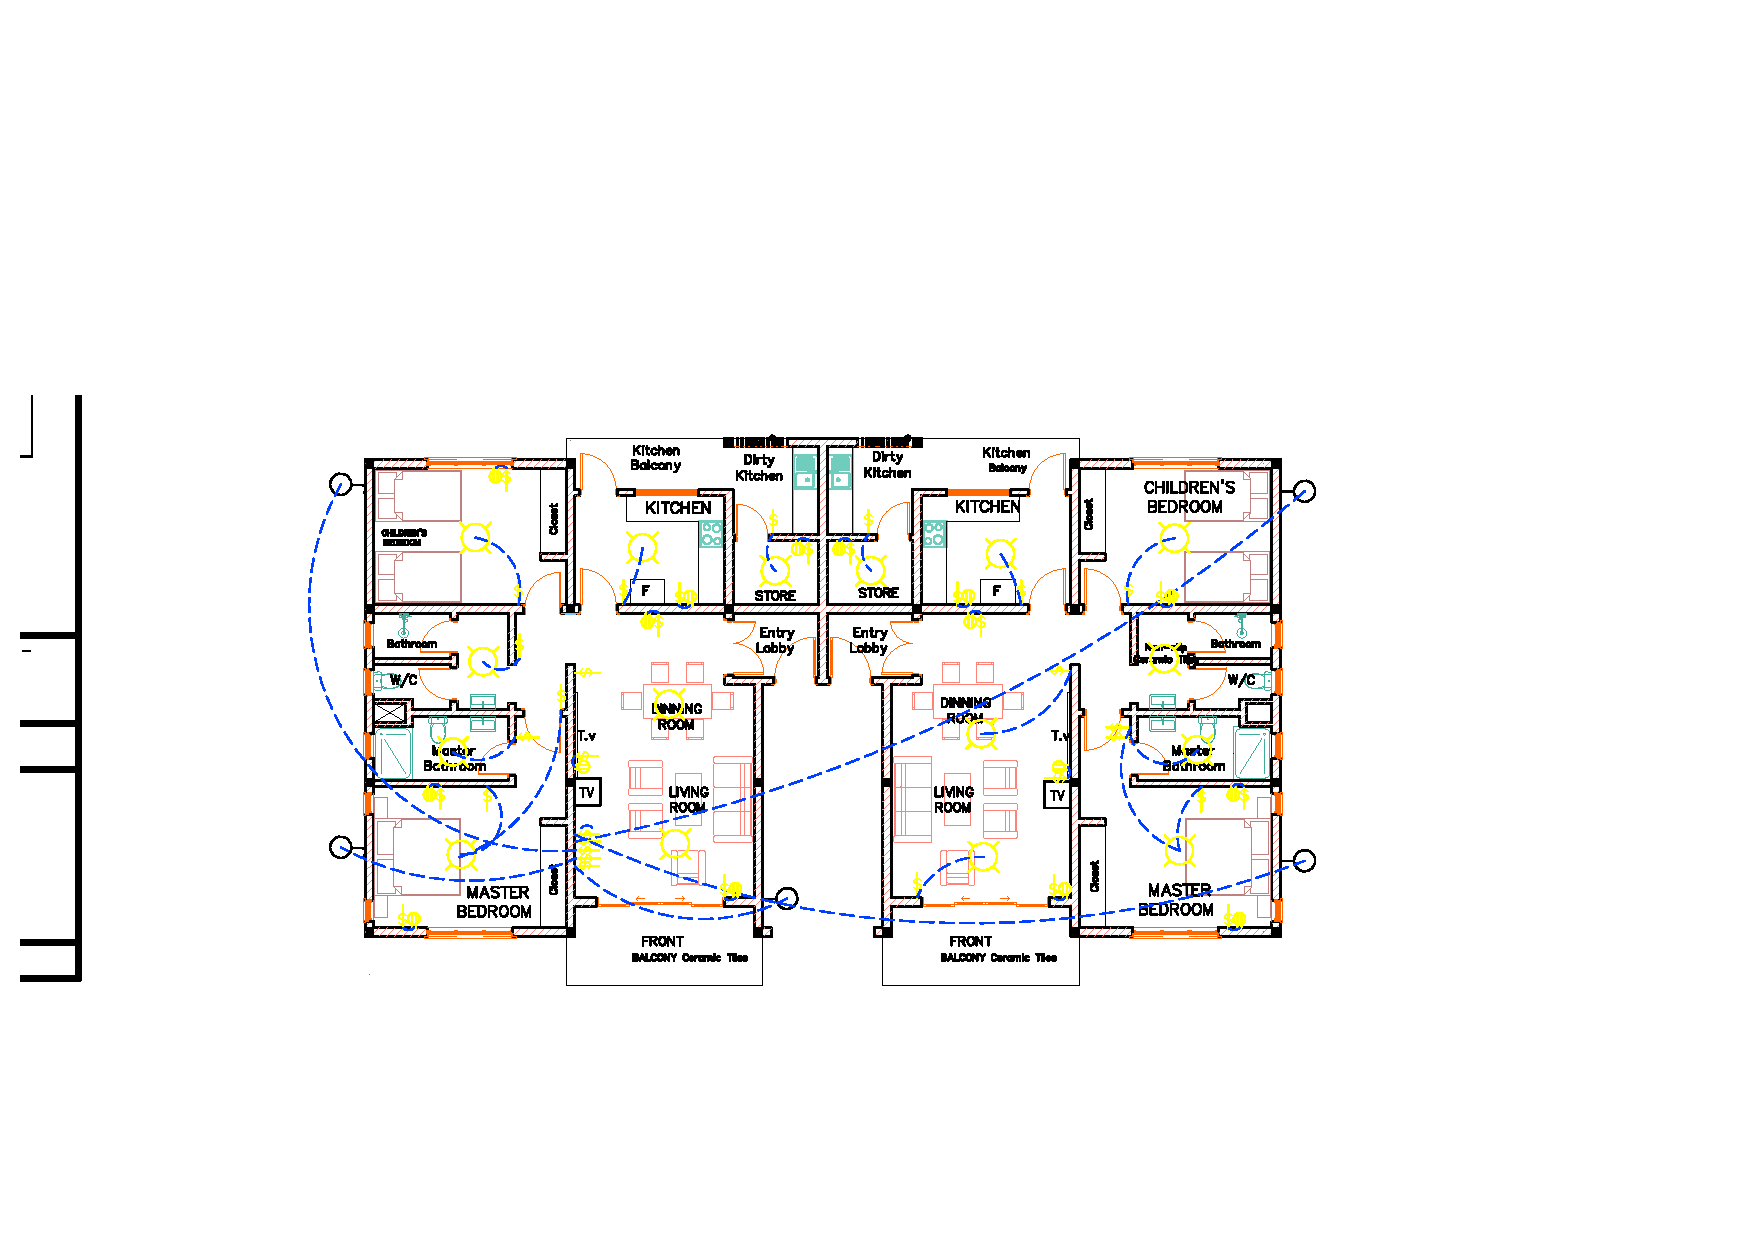
\includepdf{final_model}
\end{document}
